% !TEX root = ../thesis.tex

\chapter{Introduction}
\label{chapter:introgen}

Recent years have seen enormous advances in the field of cosmology. Thanks to technological advancements, wide-field galaxy surveys have helped mapping the universe, in particular provide high-precision data on the distribution of galaxies. From the earliest realisations that these observed galaxies can be used to trace the underlying matter density fields, the field of LSS research has been transformed into a data-driven science. 

Next-generation large-scale surveys will be able to observe at unprecedented precision. The work in this thesis was undertaken in an effort to improve the theoretical description of the statistical models used to interpret these upcoming datasets in an as unbiased manner as possible. To start, in this chapter we introduce the standard cosmological model, $\Lambda$CDM, and briefly discuss the observational evidence supporting the standard model of cosmology. We also discuss structure formation in the universe, and introduce galaxy statistics, which has been the crucial tool for studying the clustering of galaxies in the universe. Up to now, the two-point correlation function, or power spectrum in Fourier space, has been a cosmologist's most reliable statistic describing the LSS and constraining cosmological parameters. We will give a brief overview of what has been achieved with the power spectrum, and introduce the galaxy bispectrum as the first of the higher-order correlation functions. 

Estuans interius ira vehementi

\todo{describe rest of chapters}

\section{The standard cosmological model}

Over the past several decades, a consensus model for describing the evolution of the universe has emerged.  Evidence for this model is provided by a variety of observations, made possible due to technological advancements, such as the measurements of the cosmic microwave background (CMB), distance measurements using Type 1a Supernovae (SNe), and large-scale structure surveys. 

This standard model for the evolution of the universe predicts that approximately 13.8 billion years ago, the universe was in a hot and dense `Big Bang' state, from which it has continued to expand since. From Type 1a SNe measurements, it has been inferred that the late-time expansion of the universe is accelerating due to an energy component referred to as `dark energy', the physical origin of which has not yet been understood, but described by some cosmological constant $\Lambda$. Approximateley 70\% of the universe's energy budget at the present day is comprised of this dark energy. The remaining amount primarily consists of `cold dark matter' (CDM), a collisionless component which makes up about 25\% of the universe's energy content. The small remaining amount is comprised of roughly 4\% of the more familiar baryonic matter, which interacts electromagnetically, and a small relativistic radiation component (photons and neutrinos). See figure~\ref{fig:contentuniverse} for an illustration of the energy components of the universe at present day. It is from these dominant energy components that the colloquial name of the standard cosmological model is derived-- it is referred to as $\Lambda$CDM.
\begin{figure}[ht]
	\centering
	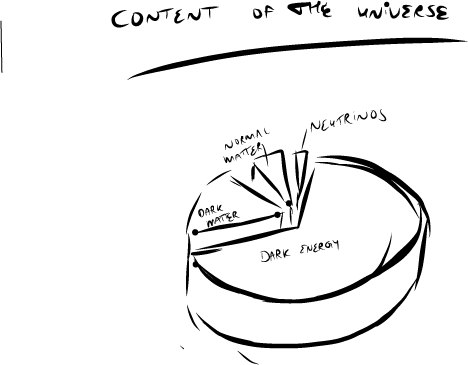
\includegraphics[width=0.6\textwidth]{fig/placeholder_universecontent.png}
	\caption{Picture of content of universe?}
	\label{fig:contentuniverse}
\end{figure}

\begin{figure}[ht]
	\centering
	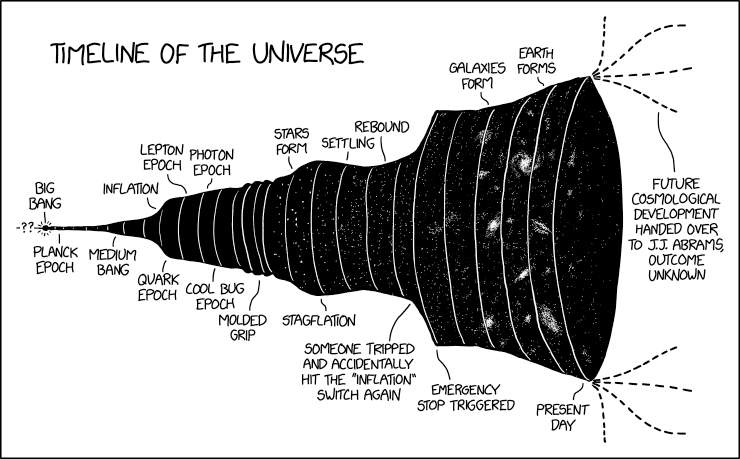
\includegraphics[width=0.6\textwidth]{fig/timeline_of_the_universe.png}
	\caption{Picture of timeline of universe?}
	\label{fig:timelineuniverse}
\end{figure}
In the 1980's, the theory of inflation was coined~\cite{Guth:1980zm,Linde:1981mu,Albrecht:1982wi}, which has since become the prevailing theory for the early universe and its initial conditions. As a theory, it successfully solves the horizon, flatness, homogeneity and isotropy problems. During inflation, the universe is expanding exponentially, rapidly increasing its scale by a factor of at least $\approx 10^{27}$. During this period of exponential expansion, quantum fluctuations are stretched to macroscopic level. These are the seeds of the cosmic structure we observe today. It is worth noting that while the properties of the universe (near homogeneous, isotropic, and spatially flat) as predicted by inflation have been confirmed observationally to very high precision, but as of yet there is no conclusive observational evidence for the inflationary model itself. 

After inflation ends, the universe cooled down, and keeps expanding though at a much slower rate than it did before. The thermal evolution of the universe is defined by the `competition' between the interaction rates of the particles and the expansion rate of the universe itself. The baryonic mass of the universe consists of approximately 75\% hydrogen ions and 25\% helium ions, plus small amounts of deuterium and lithium, all of which are created through Big Bang nucleosynthesis. Electrons, protons, and neutrinos are also present, and the charged baryonic matter is tightly coupled by electromagnetic interaction. Furthermore, the free electrons are tightly coupled also, to the photons, via Thompson scattering. All of this results in the so-called photon-baryon fluid. The pressure of this fluid prevents the fluctuations from gravitationally collapsing, which leads instead to the generation of acoustic waves. These are known as the Baryon Acoustic Oscillations (BAO), propagating until the protons and baryons decouple. This occurs around the time of `recombination' around 400,000 years after the Big Bang. At recombination, the universe has cooled down sufficiently for neutral hydrogen to form, and the now decoupled photons can free stream from the `surface of last scattering' through the universe. This background radiation, the `first light' of the universe, can be observed today-- it is known as the Cosmic Microwave Background (CMB), and primordial fluctuation patterns are imprinted on the temperature fluctuations of the CMB. 

Around 50,000 years after the Big Bang, the universe became matter-dominated. Under matter domination, the primordial density fluctuations grow due to gravitational instability. This gravitational collapse eventually leads to the formation of the cosmic web, which is a non-linear structure formed by halos, voids, and filaments, dominated by CDM. \todo{add picture?} Baryonic matter inside these dark matter halos cools down, collapses, and goes on to form stars and galaxies. Formation of this large scale structure is hierarchical, as smaller objects form first and merge to into larger structures. The resulting evolution of structure can be well-described by a linear description of perturbations on large scales (of about 150Mpc), but the small-scale nonlinearities of the fluctuations pose serious theoretical challenges.




\section{Formation of structure}

Fluctuations in early universe leading to formation of structure?


\section{Statistics of galaxy clustering}
\label{section:introbisp}

Desciption of the role of statistics in cosmology

The galaxy bispectrum is the Fourier-space equivalent of the three-point function and is as such the first of the higher-order statistics beyond the power spectrum. Next-generation large scale structure such as Euclid (galaxy) and the SKA (21cm intensity mapping) will rely on a combination of the power spectrum and the bispectrum for high-precision measurements of primordial non-Gaussianity and for improvement of constraints on cosmological parameters. In particular, improvement on constraints on the primordial non-Gaussian parameter $\fnl$ will be crucial for discrimitation between various models of inflation and other theories of the early universe. 

As it stands, our current understanding of the universe is that large scale structure of matter is a result of the growth of small primordial fluctuations which have functioned as seeds for structure growth in an otherwise homogeneous universe. These small fluctuations have been amplified by gravitatational instability, resulting in the formation of the structure that we know as the cosmic web on cosmological scales. Tests of theories describing these primordial fluctuations are statistical in nature for the following reasons. For one, there is no direct observationa access to primordial fluctuations, and additionally, the time-scales required to follow cosmological evolution of systems is much much longer than that over which observations are realistically possible. In essence this means that observations on the past lightcone how different objects at different phases of their evolution, and as a result tests of the evolution of large scale structure must be carried out statistically. 

A goal of theoretical cosmology is to make statistical predictions which depend on the statistical properties of primordial perturbations, which in turn lead to the formation of large scale structures in the universe. In these models, the observable universe is modelled simply as a stochastic realisation of a statistical ensemble of possibilities. The most widely considered models are based on the inflationary paradism, and generically give rise to adiabatic Gaussian initial fluctuations. In this case, the origin of stochasticity lies in quantum fluctuations that were generated in the early universe. 

\section{The two-point function}

A purely Gaussian field is fully described by the two-point correlation function or power spectrum. The two-point correlation function is defined as the joint ensemble average of the density at two different points $\x$ and $\x + \textbf{r}$, i.e. 
\begin{equation}
	\xi(r) = \langle \delta(\x) \delta(\x + \textbf{r}) \rangle,
\end{equation}
which is dependent on the distance $r$ between the two points only, due to statistical homogeneity and isotropy which are assumed throughout. Usually, the density contrast $\delta$ is expressed in terms of its Fourier space components, where our Fourier convention is 

\begin{equation}
	\delta({\x}) = \int \frac{\diff^3k}{(2\pi)^3} \, e^{\i \k \cdot \x } \delta(\x),
\end{equation}
where $\delta(\k)$ are complex random variables. Note that there are generally two Fourier conventions that are used in literature on the galaxy statistics, which lead to a difference of $(2\pi)^3$ in the definition of the power spectrum or two-point function. The other choice of Fourier convention is to reverse where the factor of $(2\pi)^3$ goes in the Fourier transforms, that is, using $f(\x) = \int \diff^3k e^{\i \k \cdot \x} f(\k) $ and $f(\k) = \int \frac{\diff^3 x}{(2\pi)^3} e^{-\i \k \cdot \x} f(\x)$ instead of our convention used here.

Since the density contrast is real, this means that we have
\begin{equation}
	\delta(k) = \delta^*(-\k).
\end{equation}

Similarly, the correlators can also be computed in Fourier space, as follows, 
\begin{equation}
	\langle \delta(\k) \delta(\k') \rangle = \int \diff^3 x \diff^3 r \langle \delta(\x) \delta(\x + \r)\rangle e^{-\i (\k + \k') \cdot \x - \i \k' \cdot \r}.
\end{equation}
This can be rewritten using the definition of the two-point correlation function as 
\begin{equation}
	\langle \delta(\k) \delta(\k') \rangle = \int \diff^3 x \diff^3 r \xi(r) e^{-\i (\k + \k') \cdot \x - \i \k' \cdot \r},
\end{equation}
and, performing one of the intregrals, 
\begin{align}
	\langle \delta(\k) \delta(\k') \rangle &= (2\pi)^3 \delta^D(\k + \k') \int \diff^3 r \xi(r) e^{\i \k \cdot \r} \\
	&\equiv (2\pi)^3 \delta^D(\k + \k') P(k),
\end{align}
where $P(k)$ is by definition the density power spectrum.

\subsection{The power spectrum}
\todo[inline]{Power spectrum introduction -- need to take from section above}

\subsection{The angular power spectrum}
\todo[inline]{$C_\ell$ stuff}

\section{The three-point function}

Higher-order correlation functions are defined as the connected part of the joint ensemble average of the density in an arbitrary number of locations. In principle it is possible define any order of correlation function like this, but they will rapidly become more computationally complex and expensive. In the case of a purely Gaussian field, the only non-vanishing connected part is the two-point correlation function. This is a direct consequence of Wick's theorem for Gaussian fields, and has a number of important consequences. Firstly it means that a purely Gaussian, statistically homogeneous and isotropic field is fully described by its two-point correlation function or power spectrum, and secondly it means that the statistical properties of any field, which is not necessarily linear, can be written in terms of combinations of two-point correlation functions -- as long as the field is built from a Gaussian field $\delta$. In a generic form, Wick's theorem can be expressed as 
\begin{align}
	&\langle \delta(\ka) \ldots \delta(\bm{k}_{2p + 1}) \rangle = 0 \nonumber \\
	&\langle \delta(\ka) \ldots \delta(\bm{k}_{2p})\rangle = \sum_{[\text{all distinct pairs}]} \prod_{[p \text{ pairs } (i,j)]} \langle \delta(\bm{k}_i) \delta(\bm{k}_j) \rangle.  
\end{align}

More concretely, this means that for a purely Gaussian field, $\langle \delta(\ka) \delta(\kb) \delta(\kc)\rangle = 0$. However, this changes in the presence of any sources of non-linearity. BLAH. An important consequence of non-linear evolution of structure is that the statistics of odd-number density fields are no longer vanishing. The leading odd-number statistic which will be non-zero in the case of non-linear evolution if the three-point correlation function or the bispectrum in Fourier space, 
\begin{equation}
	\langle \delta(\ka) \delta(\kb) \delta(\kc) \rangle = (2 \pi )^3 \delta^\mathrm{D}(\ka + \kb + \kc) \left[ 2 F_2(\ka,\kb) P_\mathrm{L}(\ka) P_\mathrm{L}(\kb) + \text{ 2 c.p.} \right]
\end{equation}
where $F_2$ is the Fourier space density evolution kernel, $P_\mathrm{L}$ is the linear power spectrum from the previous discussion, and redshift dependence is suppressed for brevity. 

Some blah blah about higher order statistics and their importance in future surveys (higher precision data, non-Gaussianities in the universe and effects that give rise to nonlinearities)

\subsection{The matter bispectrum}

The bispectrum is a non-Gaussian statistic, and as such is especially sensitive to any forms of non-linearity in the universe. It is an essential probe for e.g. primordial non-Gaussianity, though there are also other sources of non-Gaussianities in the universe. Primordial non-Gaussianity, which is often parametrised by the non-linear parameter $\fnl$, is predicted by different types of inflation and other theories of the early universe; meaning that improvement of constraints on $\fnl$ could help discriminate between these theories and help shed light on the very early universe and the seeds of structure formation. 

In this section we will go into more detail as to how various amplitudes and signs of the bispectrum correspond to real-space signatures. The bispectrum in Fourier space forms a closed triangle correlating three different wave-vectors and, unlike the power spectrum or two-point function, is able to correlate different scales. The matter bispectrum is unique from the thus far more well-studied CMB bispectrum in that it is able to form a three-dimensional map of the universe, whereas the cosmic microwave background provides a two-dimensional snapshot of the first light only. It is therefore essential to try and improve the theoretical description of the matter bispectrum if we are to utilise the wealth of information from next-generation high-precision galaxy surveys in as good and as unbiased a manner as possible. 

Where the power spectrum is a measure of probability of, e.g. in the case of the galaxy power spectrum, finding galaxies at distance corresponding to separation of points $r$ from each other, the bispectrum similarly maps this to a probability in a three-dimensional equivalent. That is, it can correspond directly to what we know as the cosmic web, and the galaxy or dark matter distributions therein. The bispectrum has degrees of freedom in both modulus of the wavevector i.e. scales of correlation, as well as the shape of the triangle itself. Different triangle shapes correspond to different real-space bispectrum signatures.

Theoretical blah about the matter bispectrum, definitions, showing how various bispectrum signals translate to real space shapes and modulations of signal

\subsection{Matter bispectrum in observations}

Bispectrum in observation -- can skip over any CMB and just focus on lss

\section{Galaxy bias}


(Very) brief overview of the relevant bias


\section{Primordial non-Gaussianity}

Types of primodial non-Gaussianity in the bispectrum, their signatures on various scales, scale dependence it introduces in the clustering bias etc. 


cum sit enim proprium \\
viro sapienti \\
supra petram ponere \\
sedem fundamenti \\
stultus ego comparor \\
fluvio labenti \\
sub eodem tramite \\
nunquam permanenti 